\documentclass{beamer}
\usepackage[utf8]{inputenc}

\usetheme{Madrid}
\usecolortheme{default}
\usepackage{amsmath,amssymb,amsfonts,amsthm}
\usepackage{txfonts}
\usepackage{tkz-euclide}
\usepackage{listings}
\usepackage{adjustbox}
\usepackage{array}
\usepackage{tabularx}
\usepackage{gvv}
\usepackage{lmodern}
\usepackage{circuitikz}
\usepackage{tikz}
\usepackage{graphicx}
\usepackage{multicol}

\setbeamertemplate{page number in head/foot}[totalframenumber]

\usepackage{tcolorbox}
\tcbuselibrary{minted,breakable,xparse,skins}

\definecolor{bg}{gray}{0.95}
\DeclareTCBListing{mintedbox}{O{}m!O{}}{%
  breakable=true,
  listing engine=minted,
  listing only,
  minted language=#2,
  minted style=default,
  minted options={%
    linenos,
    gobble=0,
    breaklines=true,
    breakafter=,,
    fontsize=\small,
    numbersep=8pt,
    #1},
  boxsep=0pt,
  left skip=0pt,
  right skip=0pt,
  left=25pt,
  right=0pt,
  top=3pt,
  bottom=3pt,
  arc=5pt,
  leftrule=0pt,
  rightrule=0pt,
  bottomrule=2pt,
  toprule=2pt,
  colback=bg,
  colframe=orange!70,
  enhanced,
  overlay={%
    \begin{tcbclipinterior}
    \fill[orange!20!white] (frame.south west) rectangle ([xshift=20pt]frame.north west);
    \end{tcbclipinterior}},
  #3,
}
\lstset{
    language=C,
    basicstyle=\ttfamily\small,
    keywordstyle=\color{blue},
    stringstyle=\color{orange},
    commentstyle=\color{green!60!black},
    numbers=left,
    numberstyle=\tiny\color{gray},
    breaklines=true,
    showstringspaces=false,
}

\title 
{4.4.25}
\date{}

\author
{SAMYAK GONDANE - AI25BTECH11029}

\begin{document}

\frame{\titlepage}

\begin{frame}{Question}
The equation of the line through $(2, -4)$ and parallel to the X axis is \underline{\hspace{2 cm}}.
\end{frame}

\begin{frame}{Solution}

Given: $\vec{p} = \myvec{2 \\ -4}$

\subsection*{Step 1: Direction and Normal Vectors}
The normal vector $\vec{n}$
\begin{align}
\vec{n} = \myvec{m \\ -1}\\
\vec{n} = \myvec{0 \\ -1}
\end{align}
\end{frame}

\begin{frame}{Solution}
\subsection*{Step 2: Dot Product Formulation}
Using the dot product form of a line:
\begin{align}
\vec{n}^T (\vec{x} - \vec{p}) = 0
\end{align}

Substitute:
\begin{align}
\myvec{0 & -1} \myvec{\vec{X} - \myvec{2 \\ -4}} = 0
\end{align}

\begin{align}
\Rightarrow \myvec{0 & -1}\vec{X} - \myvec{0 & -1}\myvec{2 \\ -4} = 0
\end{align}

\begin{align}
\Rightarrow \myvec{0 & -1}\vec{X} = -4
\end{align}
\end{frame}

\begin{frame}{Solution}
\textbf{Final Answer}
\begin{align}
\boxed{\myvec{0 & -1}\vec{X} = -4}
\end{align}
\end{frame}

\begin{frame}{Plot}
    \begin{figure}
        \centering
        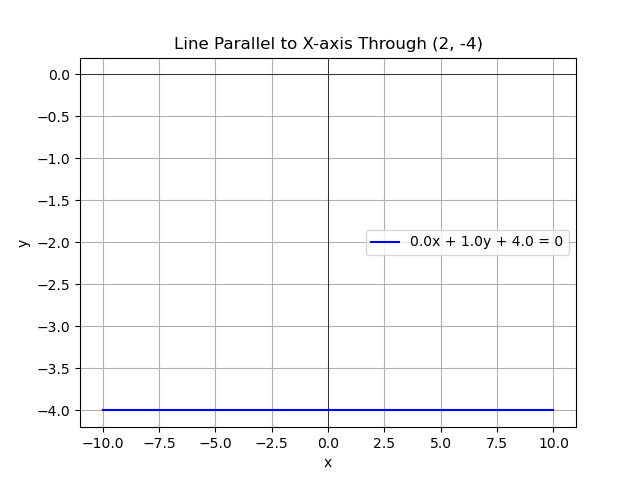
\includegraphics[width=0.5\linewidth]{./figs/Figure_1.png}
        \caption{}
        \label{fig:fig1}
    \end{figure}
\end{frame}


\end{document}